\section{The Game Loop}

\begin{center}
	\textbf{Get in cardboard box $\rightarrow$ Snake around $\rightarrow$ Profit?}
\end{center}

\lipsum[7] \cite{WikiGameLoop}

\section{Player Mechanics}

\subsection{Movement}

\lipsum[8]

\subsection{Thirst System}

\begin{figure}[H]
	\centering
	\begin{subfigure}[b]{0.45\textwidth}
		\centering
		\includegraphics[width=\textwidth]{example-image-a}
		\caption{Thirsty}
	\end{subfigure}
	\hfill
	\begin{subfigure}[b]{0.45\textwidth}
		\centering
		\includegraphics[width=\textwidth]{example-image-b}
		\caption{No Thirsty!}
	\end{subfigure}
	\caption{Drinking water is beneficial to your health!}
	\label{fig:thirst_system}
\end{figure}

\subsection{Weapon Statistics}

\lipsum[10]

\begin{table}[H]
	\centering
	\begin{tabularx}{\textwidth}{l X c c} 
		\toprule
		\textbf{Weapon Type} & \textbf{Special Ability} & \textbf{Damage} & \textbf{Speed} \\
		\midrule
		Iron Sword   & Cleave (AoE)             & 15              & 1.2s           \\
		Oak Bow      & Eagle Eye (Zoom)         & 12              & 0.8s           \\
		Stone Staff  & Mana Well (Regen)        & 20              & 2.5s           \\
		\bottomrule
	\end{tabularx}
	\caption{Base statistics for tier-1 weapons.}
	\label{tab:weapon_stats}
\end{table}

\section{Game Systems}

\lipsum[11]

\subsection{Economy Balancing}

\begin{figure}[H]
	\centering
	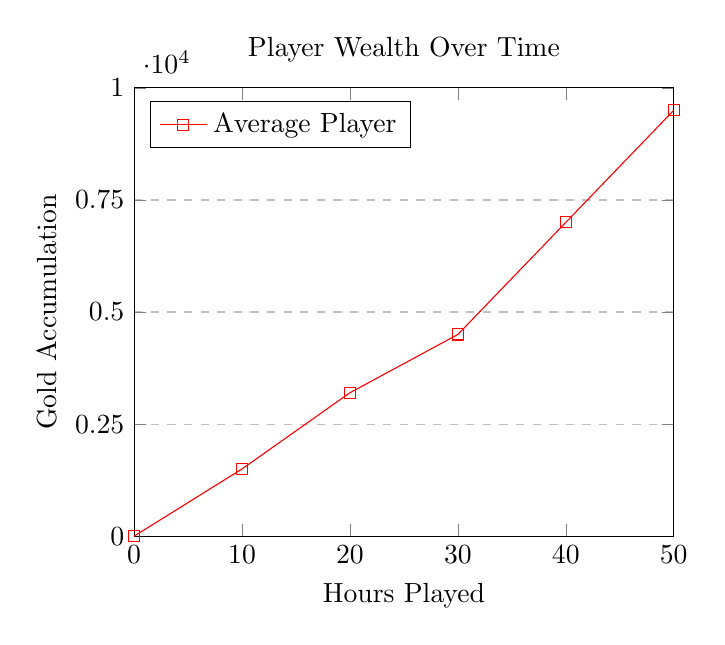
\begin{tikzpicture}
		\begin{axis}[
			title={Player Wealth Over Time},
			xlabel={Hours Played},
			ylabel={Gold Accumulation},
			xmin=0, xmax=50,
			ymin=0, ymax=10000,
			xtick={0,10,20,30,40,50},
			ytick={0,2500,5000,7500,10000},
			legend pos=north west,
			ymajorgrids=true,
			grid style=dashed,
			]
			
			\addplot[color=red, mark=square]
			coordinates {(0,0)(10,1500)(20,3200)(30,4500)(40,7000)(50,9500)};
			\addlegendentry{Average Player}
			
		\end{axis}
	\end{tikzpicture}
	\caption{Expected economy curve for a standard playthrough.}
\end{figure}

\lipsum[12]